\documentclass[aps,prb,twocolumn,groupedaddress,nofootinbib,floatfix]{revtex4}
\usepackage{graphicx}
\usepackage{graphics}
\usepackage{epsfig}
\usepackage{url}
\usepackage[utf8]{inputenc}
\usepackage[T1]{fontenc}
\usepackage{textcomp}
\usepackage{amsmath, amssymb}
\usepackage[at]{easylist}
\usepackage{soul}

\pdfsuppresswarningpagegroup=1

\begin{document}
\title{Photoelectric Effect}
\author{Preston Seligman}

\affiliation{Tulane University, Physics and Engineering Physics.}



\date{February 16, 2025}

\begin{abstract} \noindent This is the homework to get acquainted with Latex. The first lab was performed on the photoelectric effect. Here is where the abstract of the lab report will go. I use vim with MiKTeX for Latex documents. 
\end{abstract}

\maketitle

\section*{Introduction}

%The asterisk makes it so the sections aren't numbered.
It is recommended that you start with an Introduction or Background
section.  When you cite things \cite{Emissivity} put the citations in the 'thebibliography' section at the bottom of this .tex file.   It is good to have both historical and modern references.



\section*{Theory}


Below are examples of how to use LaTeX.  You will need to update with any equations you use.

My favorite equation would have to be the Zimm Equation for Static Light Scattering, which can be written as


\begin{equation}
\frac{K_{c}}{R}=\frac{1}{M_{W}}+2A_{2}c+3A_{3}c^2\ldots
\label{eq:Zimm}
\end{equation}

where $K_{c}$ is a constant that depends on solvent properties, wavelength, and angle of incidence. Equation \ref{eq:Zimm} can therefore be used to plot, after SLS data collection, and where particle size is $<\frac{\lambda}{20}$, a Debeye plot, in which the intercept of the slope is the $M_{w}$ weight-average molecular weight of the polymer in solution, and the slope of the graph is $A_{2}$ the second virial coefficient, an important material property. This equation, whilst complex, is so versatile that it can represent important material properties in an elegant and easily determinable way.


\subsection*{Your first subsection}
You can use subsections if you want. They are not REQUIRED


\section*{Experiment}

You can describe the equipment and what you did here.   
If you want to show the data in a table this is an example of how to create one. TABLES ARE NOT REQUIRED. Tables are useful for showing summaries of results, but do NOT put in data tables of your raw data. That is sometimes available in the supplementary information.

\begin{table}[h!]
\begin{center}
 \begin{tabular}{||c |||c c| c||} 
 \hline
 Col1 & Col2 & Col2 & Col3 \\
 \hline\hline
 1 & 6 & 87837 & 787 \\ 
 \hline
 2 & 7 & 78 & 5415 \\
 \hline
 3 & 545 & 778 & 7507 \\
 \hline
\end{tabular}
\label{tab:dumbdata}
\caption{This data is meaningless}
\end{center}
\end{table}

\section*{Analysis}

You will have figures in this paper (and not just in the analysis section).  Put figures where they belong, in the sections above.   \textbf{Figures must be your own, or you must cite the source.}  


{\bf Lists!}
\begin{itemize}\itemsep1pt \parskip0pt 
\item You
\item Might
\item Make
\item A
\item List
\end{itemize}
\begin{easylist}
	@ I can also use easylist
	@@ To make a list like this
	@@@ With easily nested groups
	@ Almost like Microsoft Word
	@@ Or Google Drive
\end{easylist}

It is crucially important that figures have large enough type font that you can read the axis labels and any insets.   Test this before preparing many figures.   It is surprisingly difficult to make the type big enough to still be readable once reduced to two-column format size.

Every figure must have a caption and a label.  You must refer to your Figures in the text itself, by saying ``Look at my beautiful figure, as seen in Figure \ref{fig:Animal}.''

This .tex file will not compile because it is asking for boat.jpg (which you don't have).

\begin{figure}[ht!]
        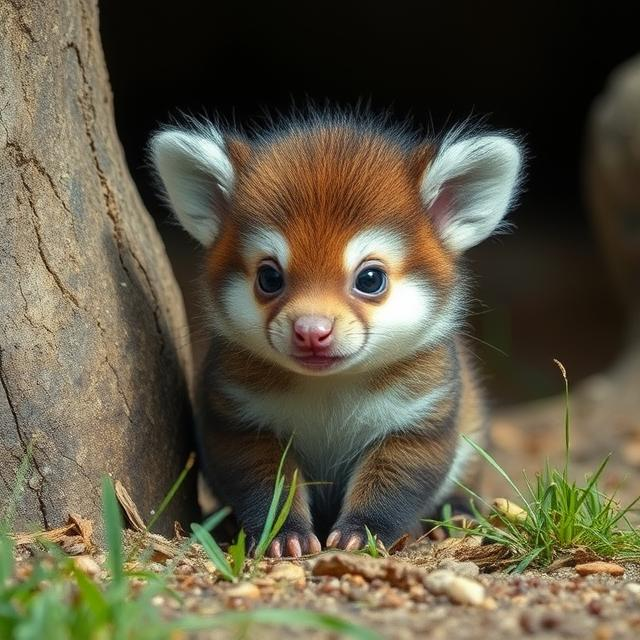
\includegraphics[width=2 in]{cute.jpg}
        \caption{AI Generation for "Cutest Animal in the World"}
        \label{fig:Animal}
\end{figure}


\section*{Acknowledgments}
Thank people who may have assisted you or discussed your experiment and/or analysis with you, but did not actually perform the experiment or analysis with you.

\begin{thebibliography}{9}

\bibitem{Emissivity}
  Infrared Emissivity Table [5 Feb. 2025]. https://www.thermoworks.com/emissivity-table/ 

\end{thebibliography}


\end{document}
